%Use one of the two documentclass lines depending on aspect ratio needed
% for 4x3 aspect ratio slides
%\documentclass{beamer}
%for 16x9 (modern wide screen) aspect ratio slides
\documentclass[aspectratio=169]{beamer}

% Oxford Maths theming
\usetheme{oxfordmaths}
\usepackage{subcaption}
\usepackage[absolute,overlay]{textpos}
\usepackage{tikz}
\usetikzlibrary{positioning}

% Set author etc info
\title[Multilevel Monte Carlo for SPDEs] %short version of title for slide footer
{Multilevel Monte Carlo for Stochastic PDEs} %full title for titlepage
\author{Inti Mantripp}
\institute{Mathematical Institute\\University of Oxford}
\date[17 Sep 2025]  %short date for slide footer
{MMSC Viva Voce, Sep 2025} %main date for title page,
                        %can overload it to show say 'Conference X, Date Y'


%% Now for the actual slides %%
\begin{document}

\begin{frame}[plain]
  \titlepage
\end{frame}

\begin{frame}
  \frametitle{Dissertation Goals}
  % \framesubtitle{A bit more information about this}
  \vspace{-0.5em}
There are three main questions my dissertation aimed to answer:

\begin{enumerate}
   \item What cost savings can MLMC achieve over standard MC 
   for two representative parabolic SPDEs?
   \item What are the effects of different coupling mechanisms?
   \item What further performance improvements can 
   parallelisation achieve?
\end{enumerate}

\end{frame}
\begin{frame}{Multilevel Monte Carlo Implementation}

 \begin{center}
    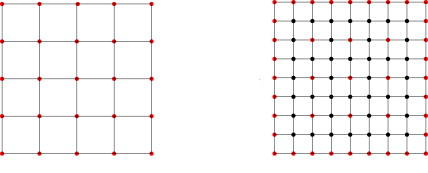
\includegraphics[height=3cm]{presentation_graphics/fine_grid_vs_coarse_grid.png}
\end{center}   

{\footnotesize
\begin{columns}[T] 
  \begin{column}{0.48\textwidth}
    \centering
    \textbf{Stochastic Heat Equation (SHE)}
    \begin{align*}
        \frac{\partial u}{\partial t} &= \frac{\partial^2 u}{\partial x^2} + \xi \\
        u(0,x) &= 0, \ u(t,0) = u(t,1) = 0 \\
        P = \int_0^1 u^2\,dx &\quad P = \Big(\int_0^1 u(x,T)\sin(n\pi x)\,dx\Big)^2
    \end{align*}
  \end{column}
  %
  \begin{column}{0.48\textwidth}
    \centering
    \textbf{Dean-Kawasaki (DK) Equation}
    \begin{align*}
        \frac{\partial \rho}{\partial t} &= \frac{1}{2}\frac{\partial^2 \rho}{\partial x^2} + N_p^{-\frac{1}{2}}\frac{\partial (\sqrt{\rho}\,\xi)}{\partial x} \\
        \rho(0,x) &= \rho_0(x), \ \text{periodic} \\
        P &= N_p \Big(\int_0^{2\pi}(\rho-\bar\rho)\sin(x)\,dx\Big)^2
    \end{align*}
  \end{column}
\end{columns}
}

    \begin{textblock*}{9cm}(4.8cm,4.5cm)
        \scalebox{0.7}{
            Coarse Mesh
        }
    \end{textblock*}
    \begin{textblock*}{9cm}(9.65cm,4.5cm)
        \scalebox{0.7}{
            Fine Mesh
        }
    \end{textblock*}
\end{frame}

\begin{frame}{Multilevel Monte Carlo Implementation}

 \begin{center}
    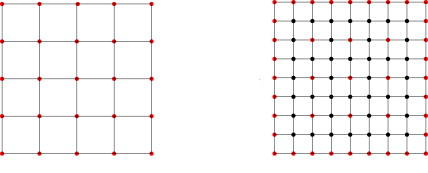
\includegraphics[height=3cm]{presentation_graphics/fine_grid_vs_coarse_grid.png}
\end{center}   

{\footnotesize
\begin{columns}[T] 
  \begin{column}{0.48\textwidth}
    \centering
    \textbf{Stochastic Heat Equation (SHE)}
    \begin{align*}
        U_j^{n+1} &= U_j^n + \lambda (U_{j+1}^n - 2U_{j}^n + U_{j-1}^n) + \Delta W_j^n 
        \vphantom{\frac{F_{j+1}^{\,n}}{2\Delta x}}
        \\
        U_j^0 &= 0, \ U_0^n = U_J^n = 0 \\
        \hat{P} &= (U^n,U^n)_{\Delta x} \quad \hat{P} = \left(U, \phi_n\right)_{\Delta x}^2
    \end{align*}
  \end{column}
  %
  \begin{column}{0.48\textwidth}
    \centering
    \textbf{Dean-Kawasaki (DK) Equation}
    \begin{align*}
        \rho_j^{\,n+1} &= \rho_j^{\,n} + \tfrac{\lambda}{2}\,\bigl(\rho_{j+1}^{\,n}-2\rho_j^{\,n}+\rho_{j-1}^{\,n}\bigr)
        + \tfrac{1}{\sqrt{N_p}}\,
        \frac{F_{j+1}^{\,n}-F_{j-1}^{\,n}}{2\Delta x} \\
        \rho_j^0 &= \rho_0(x_j), \quad \rho_0^n = \rho_J^n, \\
        P &= N_p \left( \big(\rho^n - \bar\rho^n,\ 
        \sin(\Delta x)\big)_{\Delta x} \right)^{\!2}
    \end{align*}
  \end{column}
\end{columns}
}

    \begin{textblock*}{9cm}(4.8cm,4.5cm)
        \scalebox{0.7}{
            Coarse Mesh
        }
    \end{textblock*}
    \begin{textblock*}{9cm}(9.65cm,4.5cm)
        \scalebox{0.7}{
            Fine Mesh
        }
    \end{textblock*}
\end{frame}

\begin{frame}{Coupling mechanisms}

    \begin{columns}[T] 
        \begin{column}{0.32\textwidth}
            \centering
            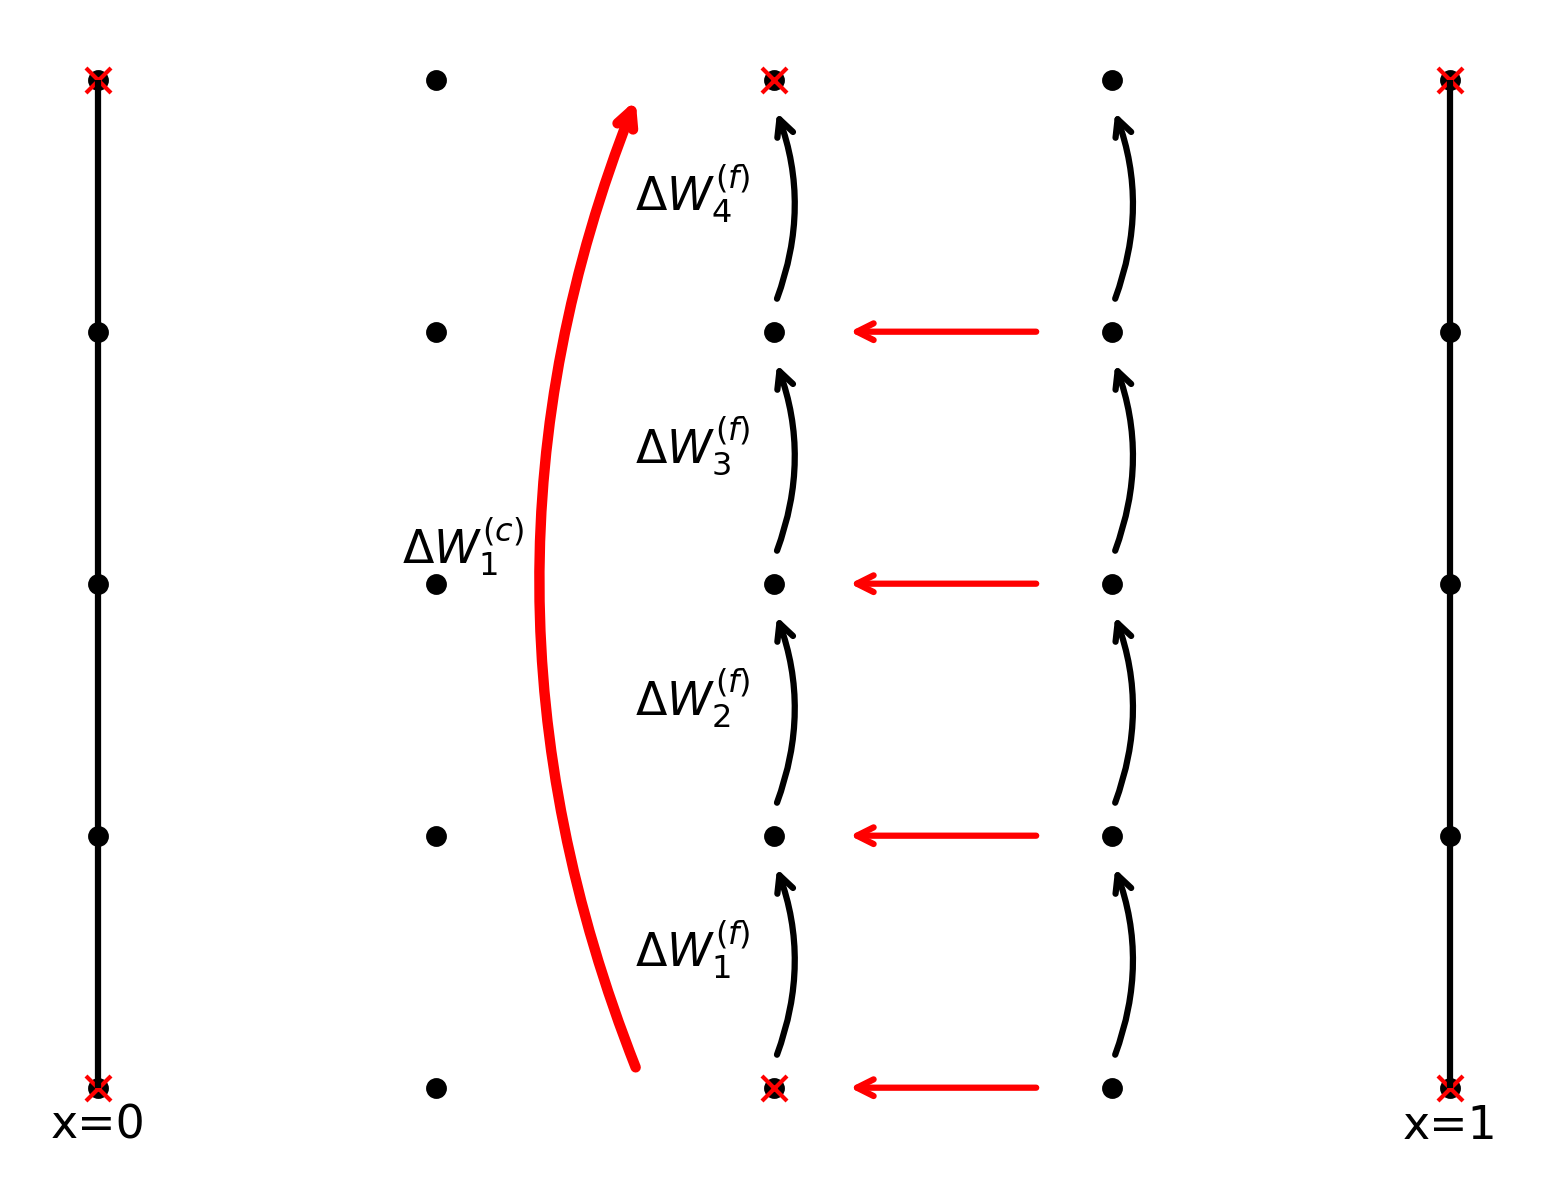
\includegraphics[width=\linewidth]{presentation_graphics/nn.png}
            {Nearest-Neighbour}
            \begin{itemize}\tiny
                \item Used by Cornalba \& Fischer.
                \item Coarse noise = sum of underlying + fine neighbour.
            \end{itemize}
        \end{column}

        \begin{column}{0.32\textwidth}
            \centering
            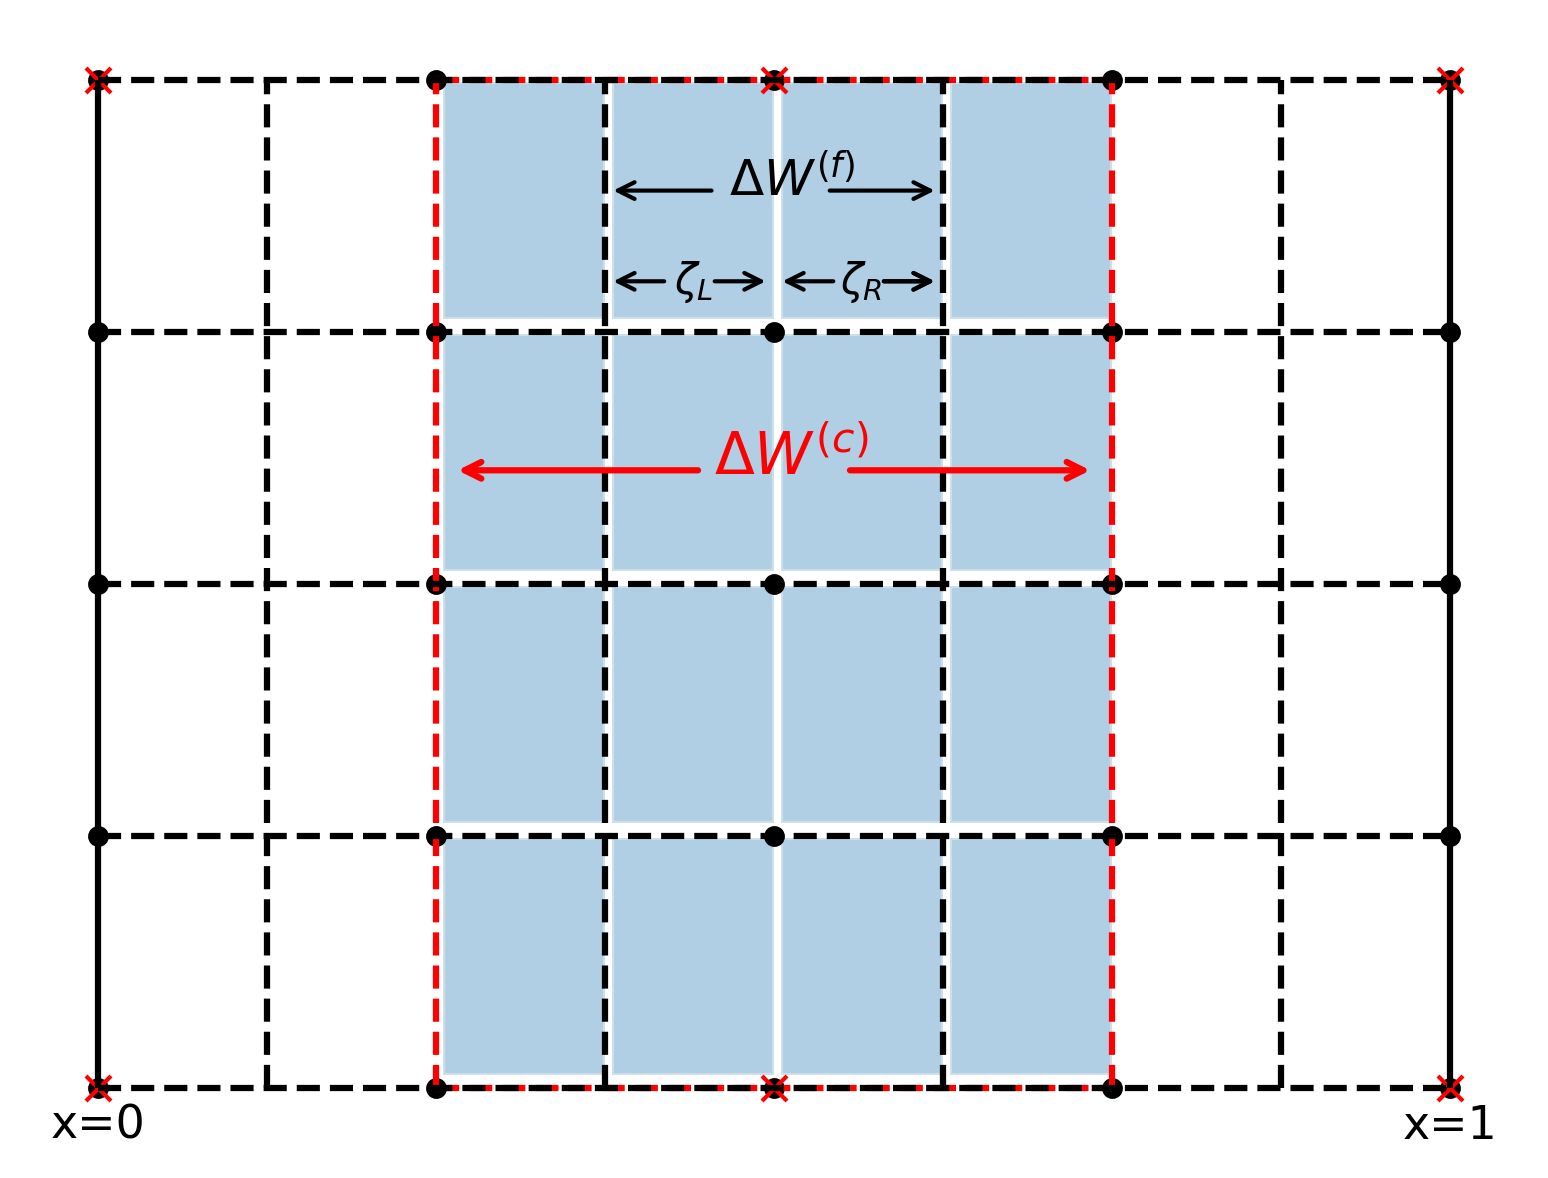
\includegraphics[width=\linewidth]{presentation_graphics/cc.png}
            {Central Coupling}
            \begin{itemize}\tiny
                \item Introduced in this dissertation.
                \item Mesh split into half-cells.
                \item Coarse noise built from shared half-cell increments.
            \end{itemize}
        \end{column}

        \begin{column}{0.32\textwidth}
            \centering
            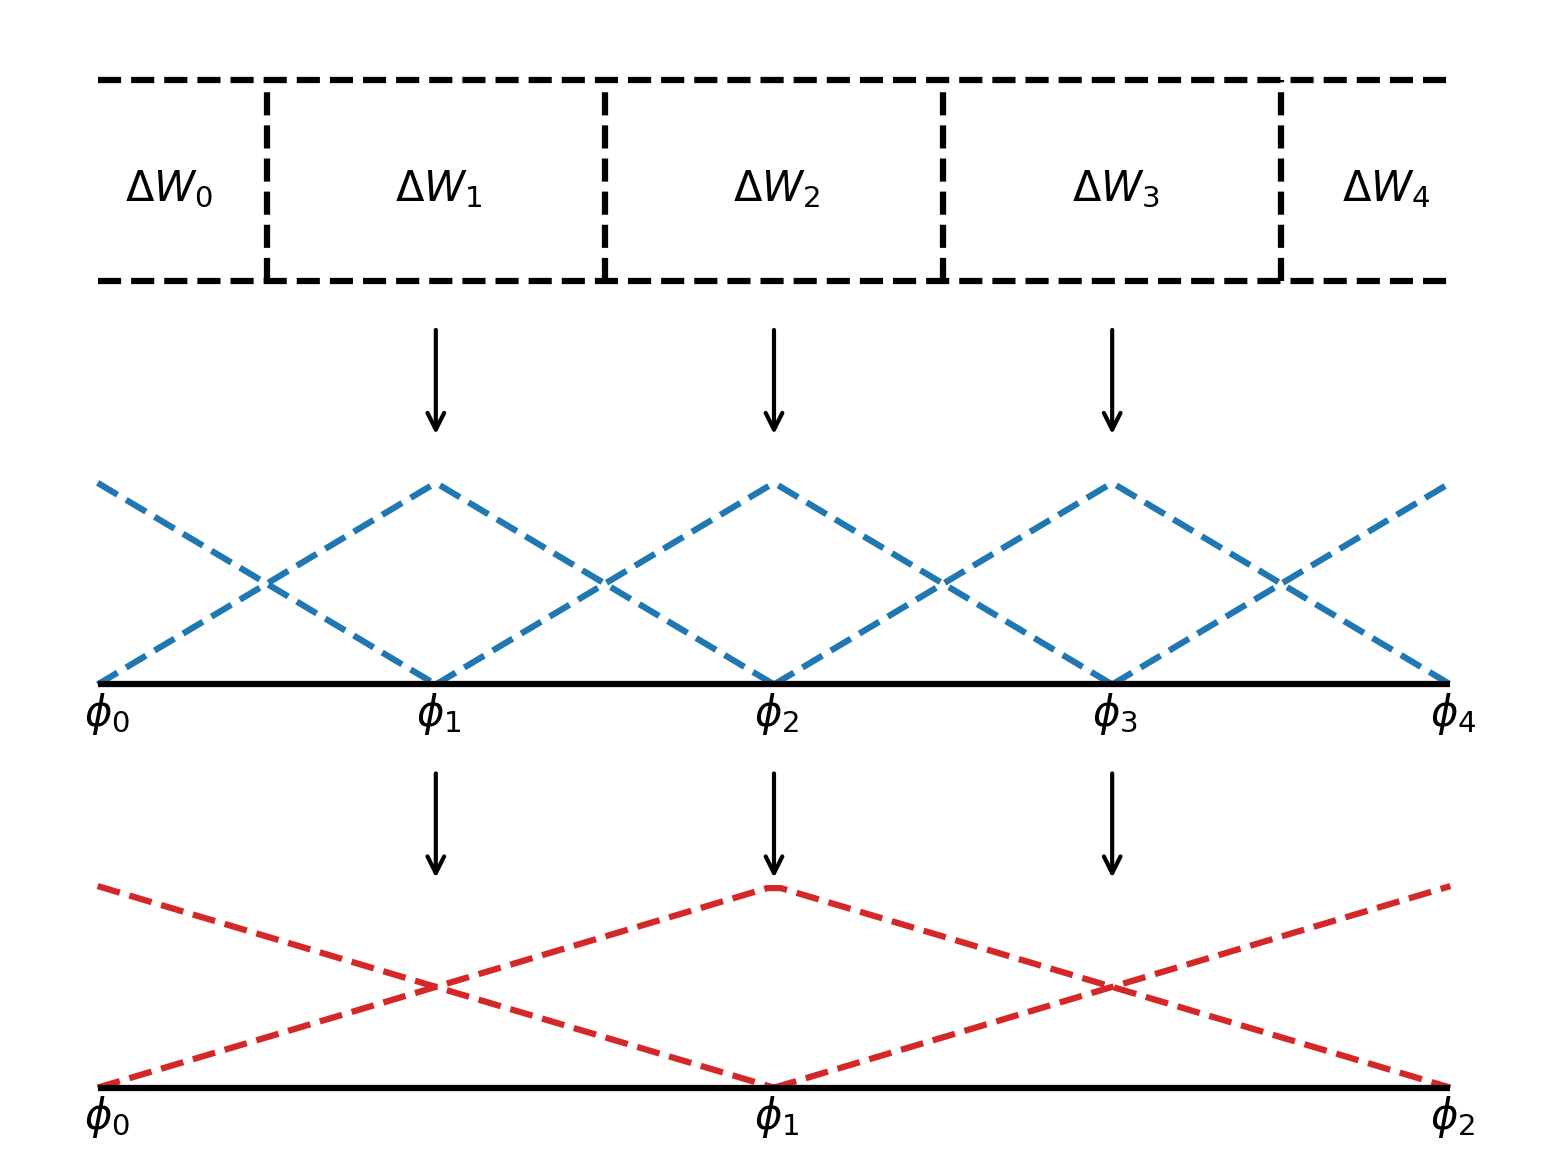
\includegraphics[width=\linewidth]{presentation_graphics/fe.png}
            {Finite Element}
            \begin{itemize}\tiny
                \item Introduced in this dissertation.
                \item Noise projected onto hat basis.
                \item Coarse hats formed as sums of fine hats.
            \end{itemize}
        \end{column}
    \end{columns}

    \begin{textblock*}{9cm}(4.9cm,5.25cm)
        \scalebox{0.4}{
            $t_c = 0,
            t_f = 0$
        }
    \end{textblock*}
    \begin{textblock*}{9cm}(4.9cm,2.35cm)
        \scalebox{0.4}{
            $t_c = 1, t_f = 4$
        }
    \end{textblock*}
\end{frame}


\begin{frame}{Effects of Coupling Mechanisms}
\begin{columns}[T] 
        \begin{column}{0.32\textwidth}
            \centering
            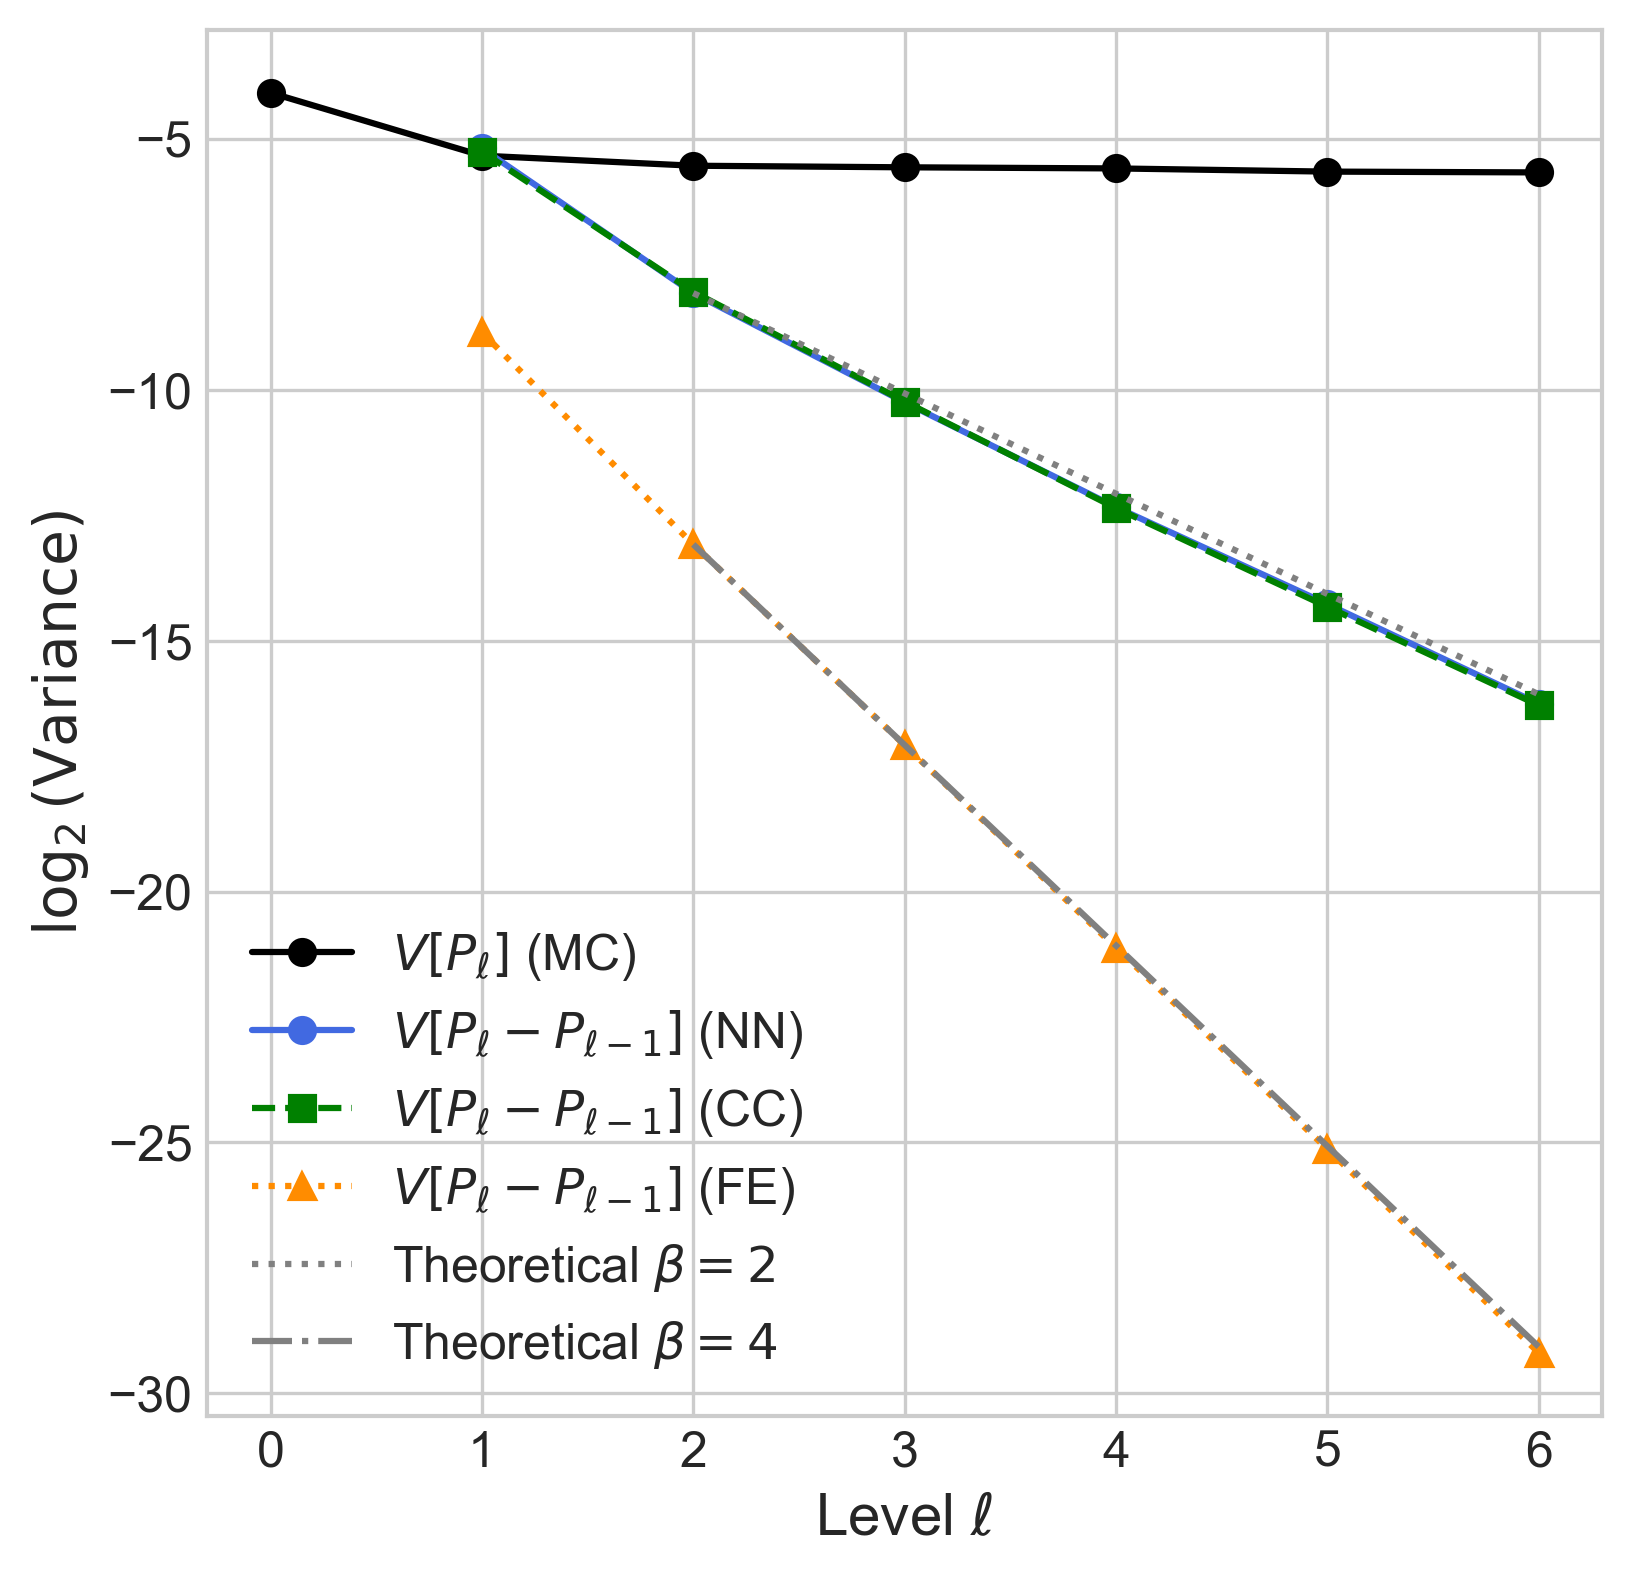
\includegraphics[width=\linewidth]{presentation_graphics/she_sq_amp_var_decay.png}
            {\scriptsize SHE - Squared Amplitude}
            \begin{itemize}\tiny
                \item CC and NN coupling equivalent
                \item FE coupling achieves improved variance decay.
            \end{itemize}
        \end{column}

        \begin{column}{0.32\textwidth}
            \centering
            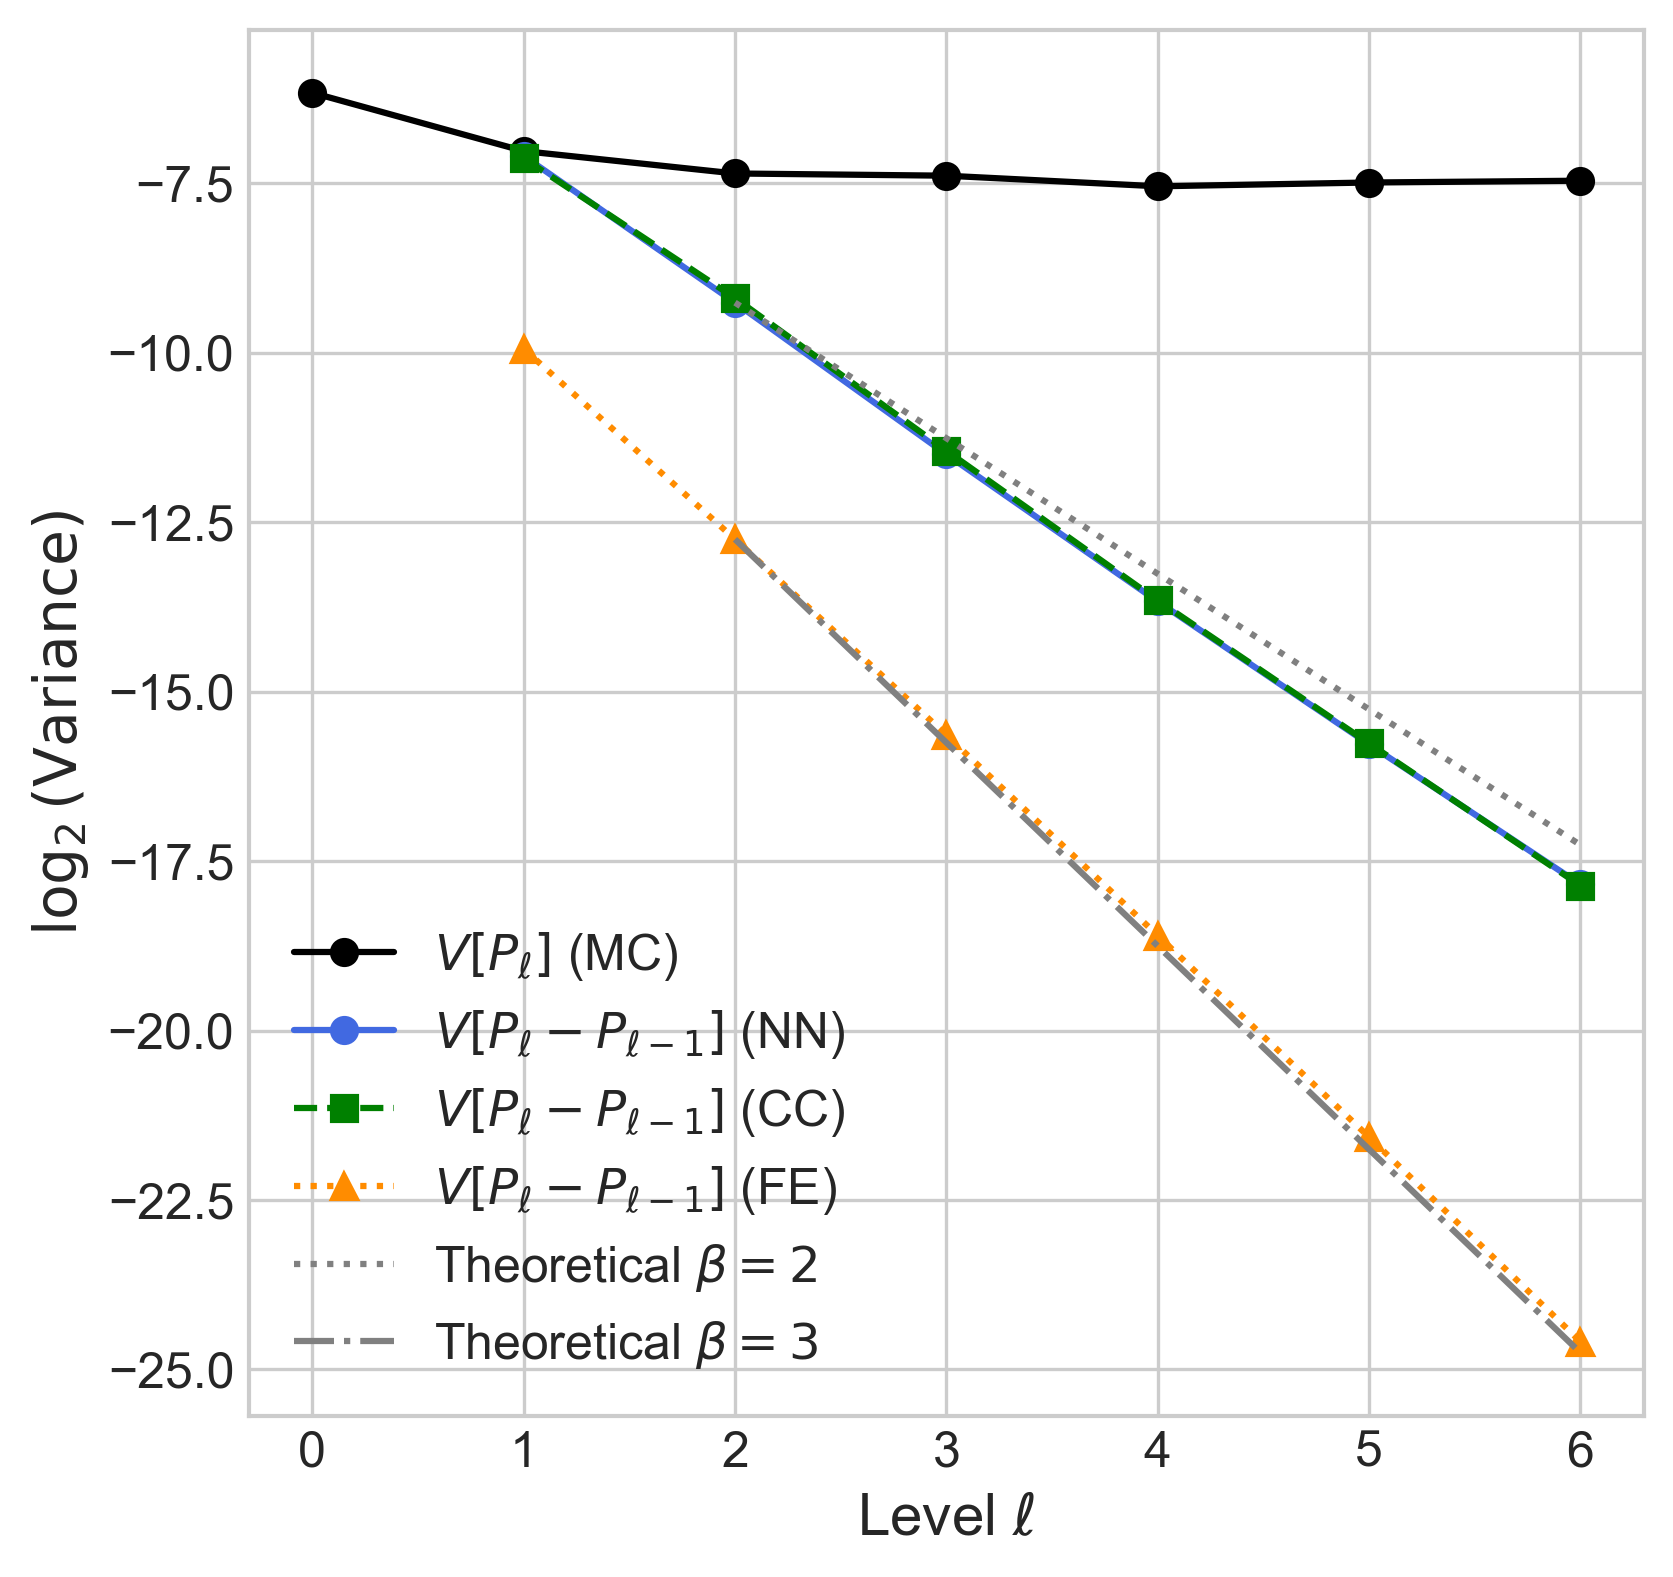
\includegraphics[width=\linewidth]{presentation_graphics/she_energy_var_decay.png}
            {\scriptsize SHE - Energy}
            \begin{itemize}\tiny
                \item CC and NN coupling equivalent.
                \item FE coupling achieves improved variance decay.
            \end{itemize}
        \end{column}

        \begin{column}{0.32\textwidth}
            \centering
            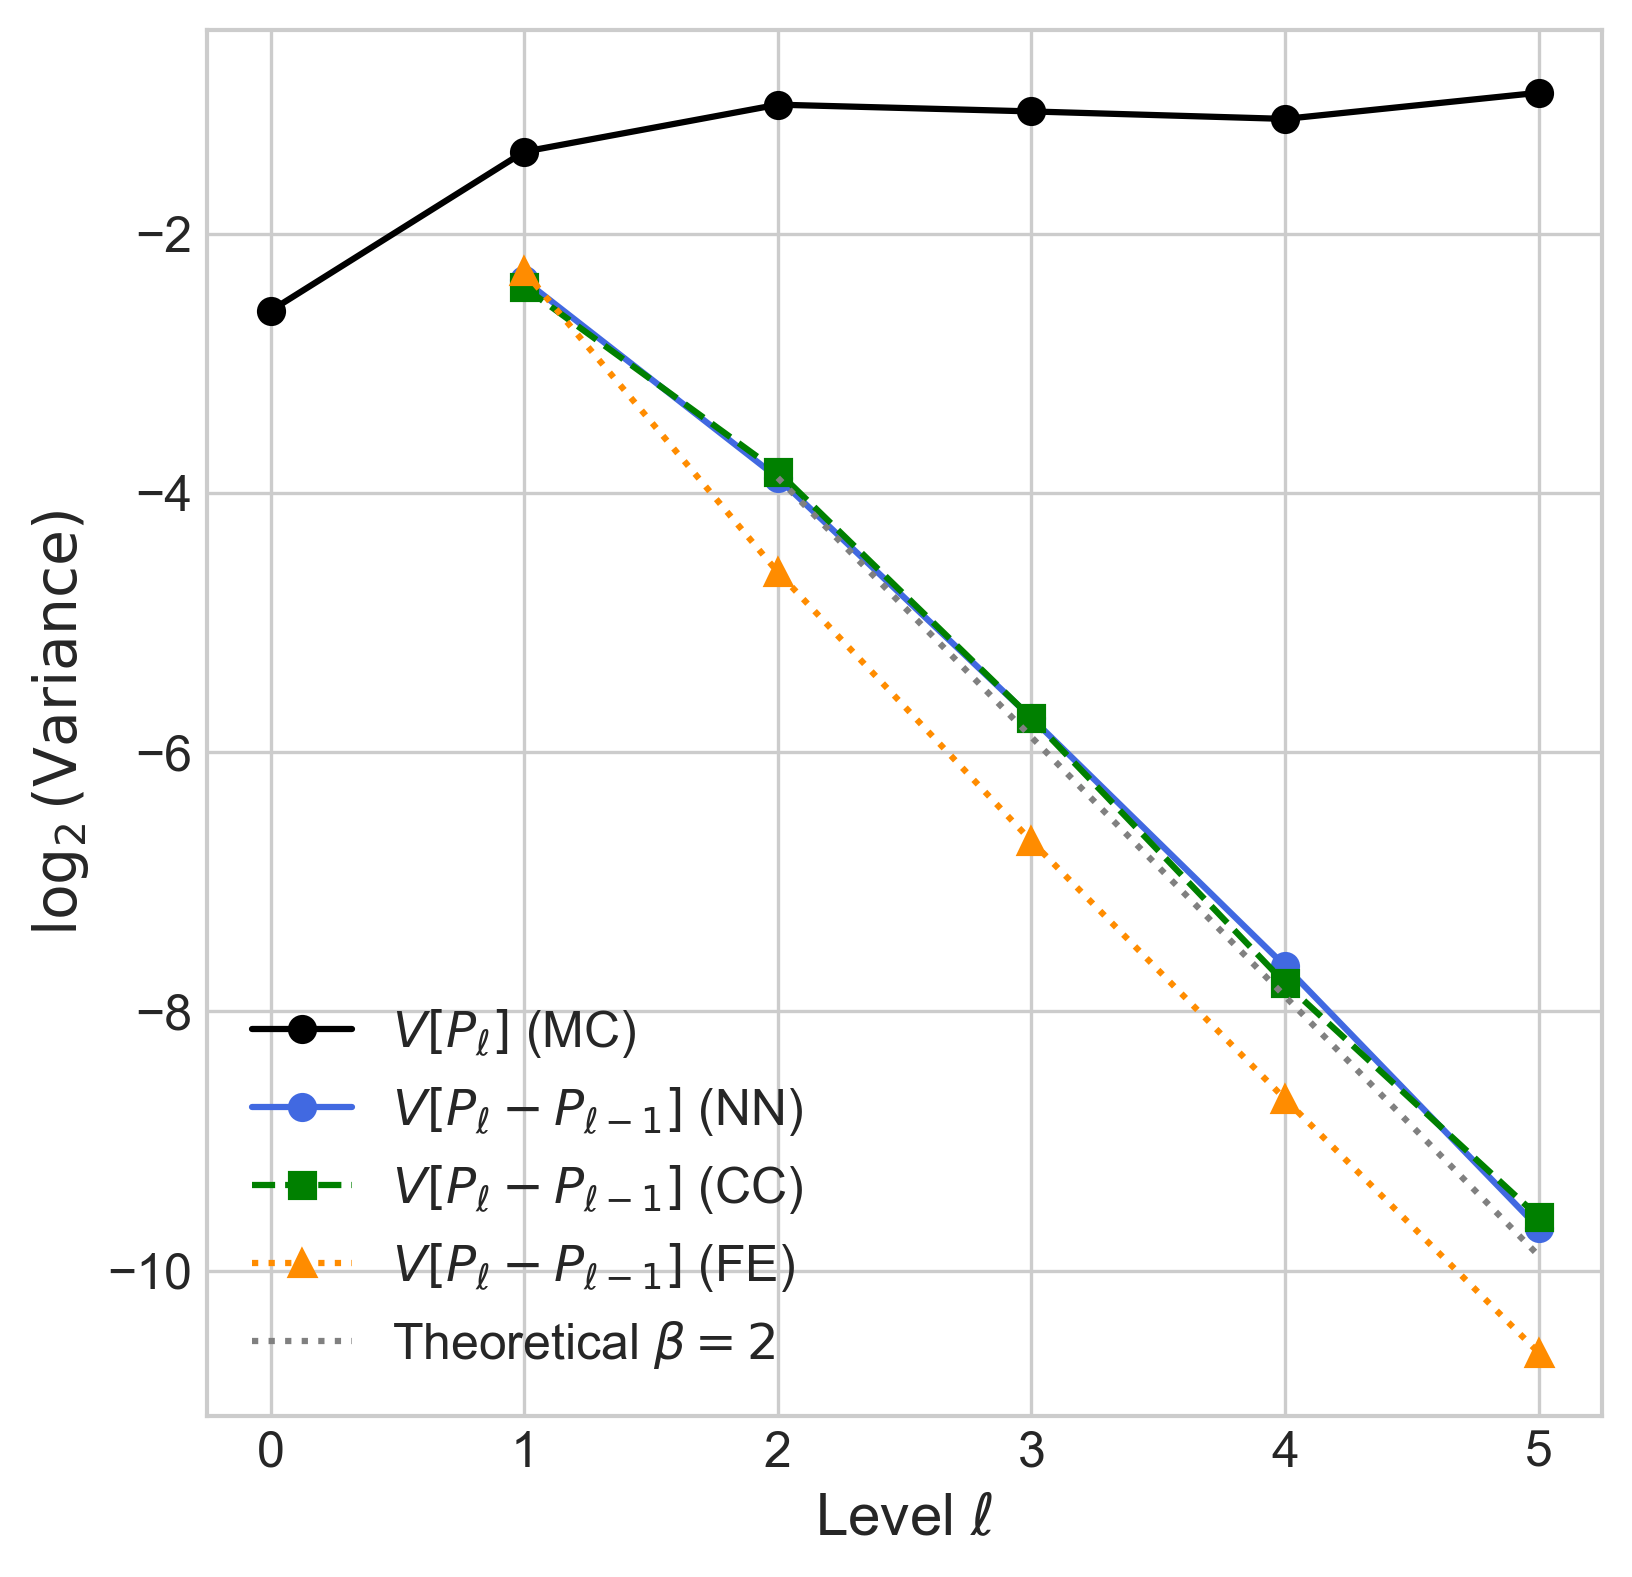
\includegraphics[width=\linewidth]{presentation_graphics/dk_var_decay.png}
            {\scriptsize DK - Mean Fluctuations}
            \begin{itemize}\tiny
                \item All coupling mechanisms achieve equivalent variance decay.
            \end{itemize}
        \end{column}
    \end{columns}

\end{frame}

\begin{frame}{Performance Results}
\begin{columns}[T] 
        \begin{column}{0.32\textwidth}
            \centering
            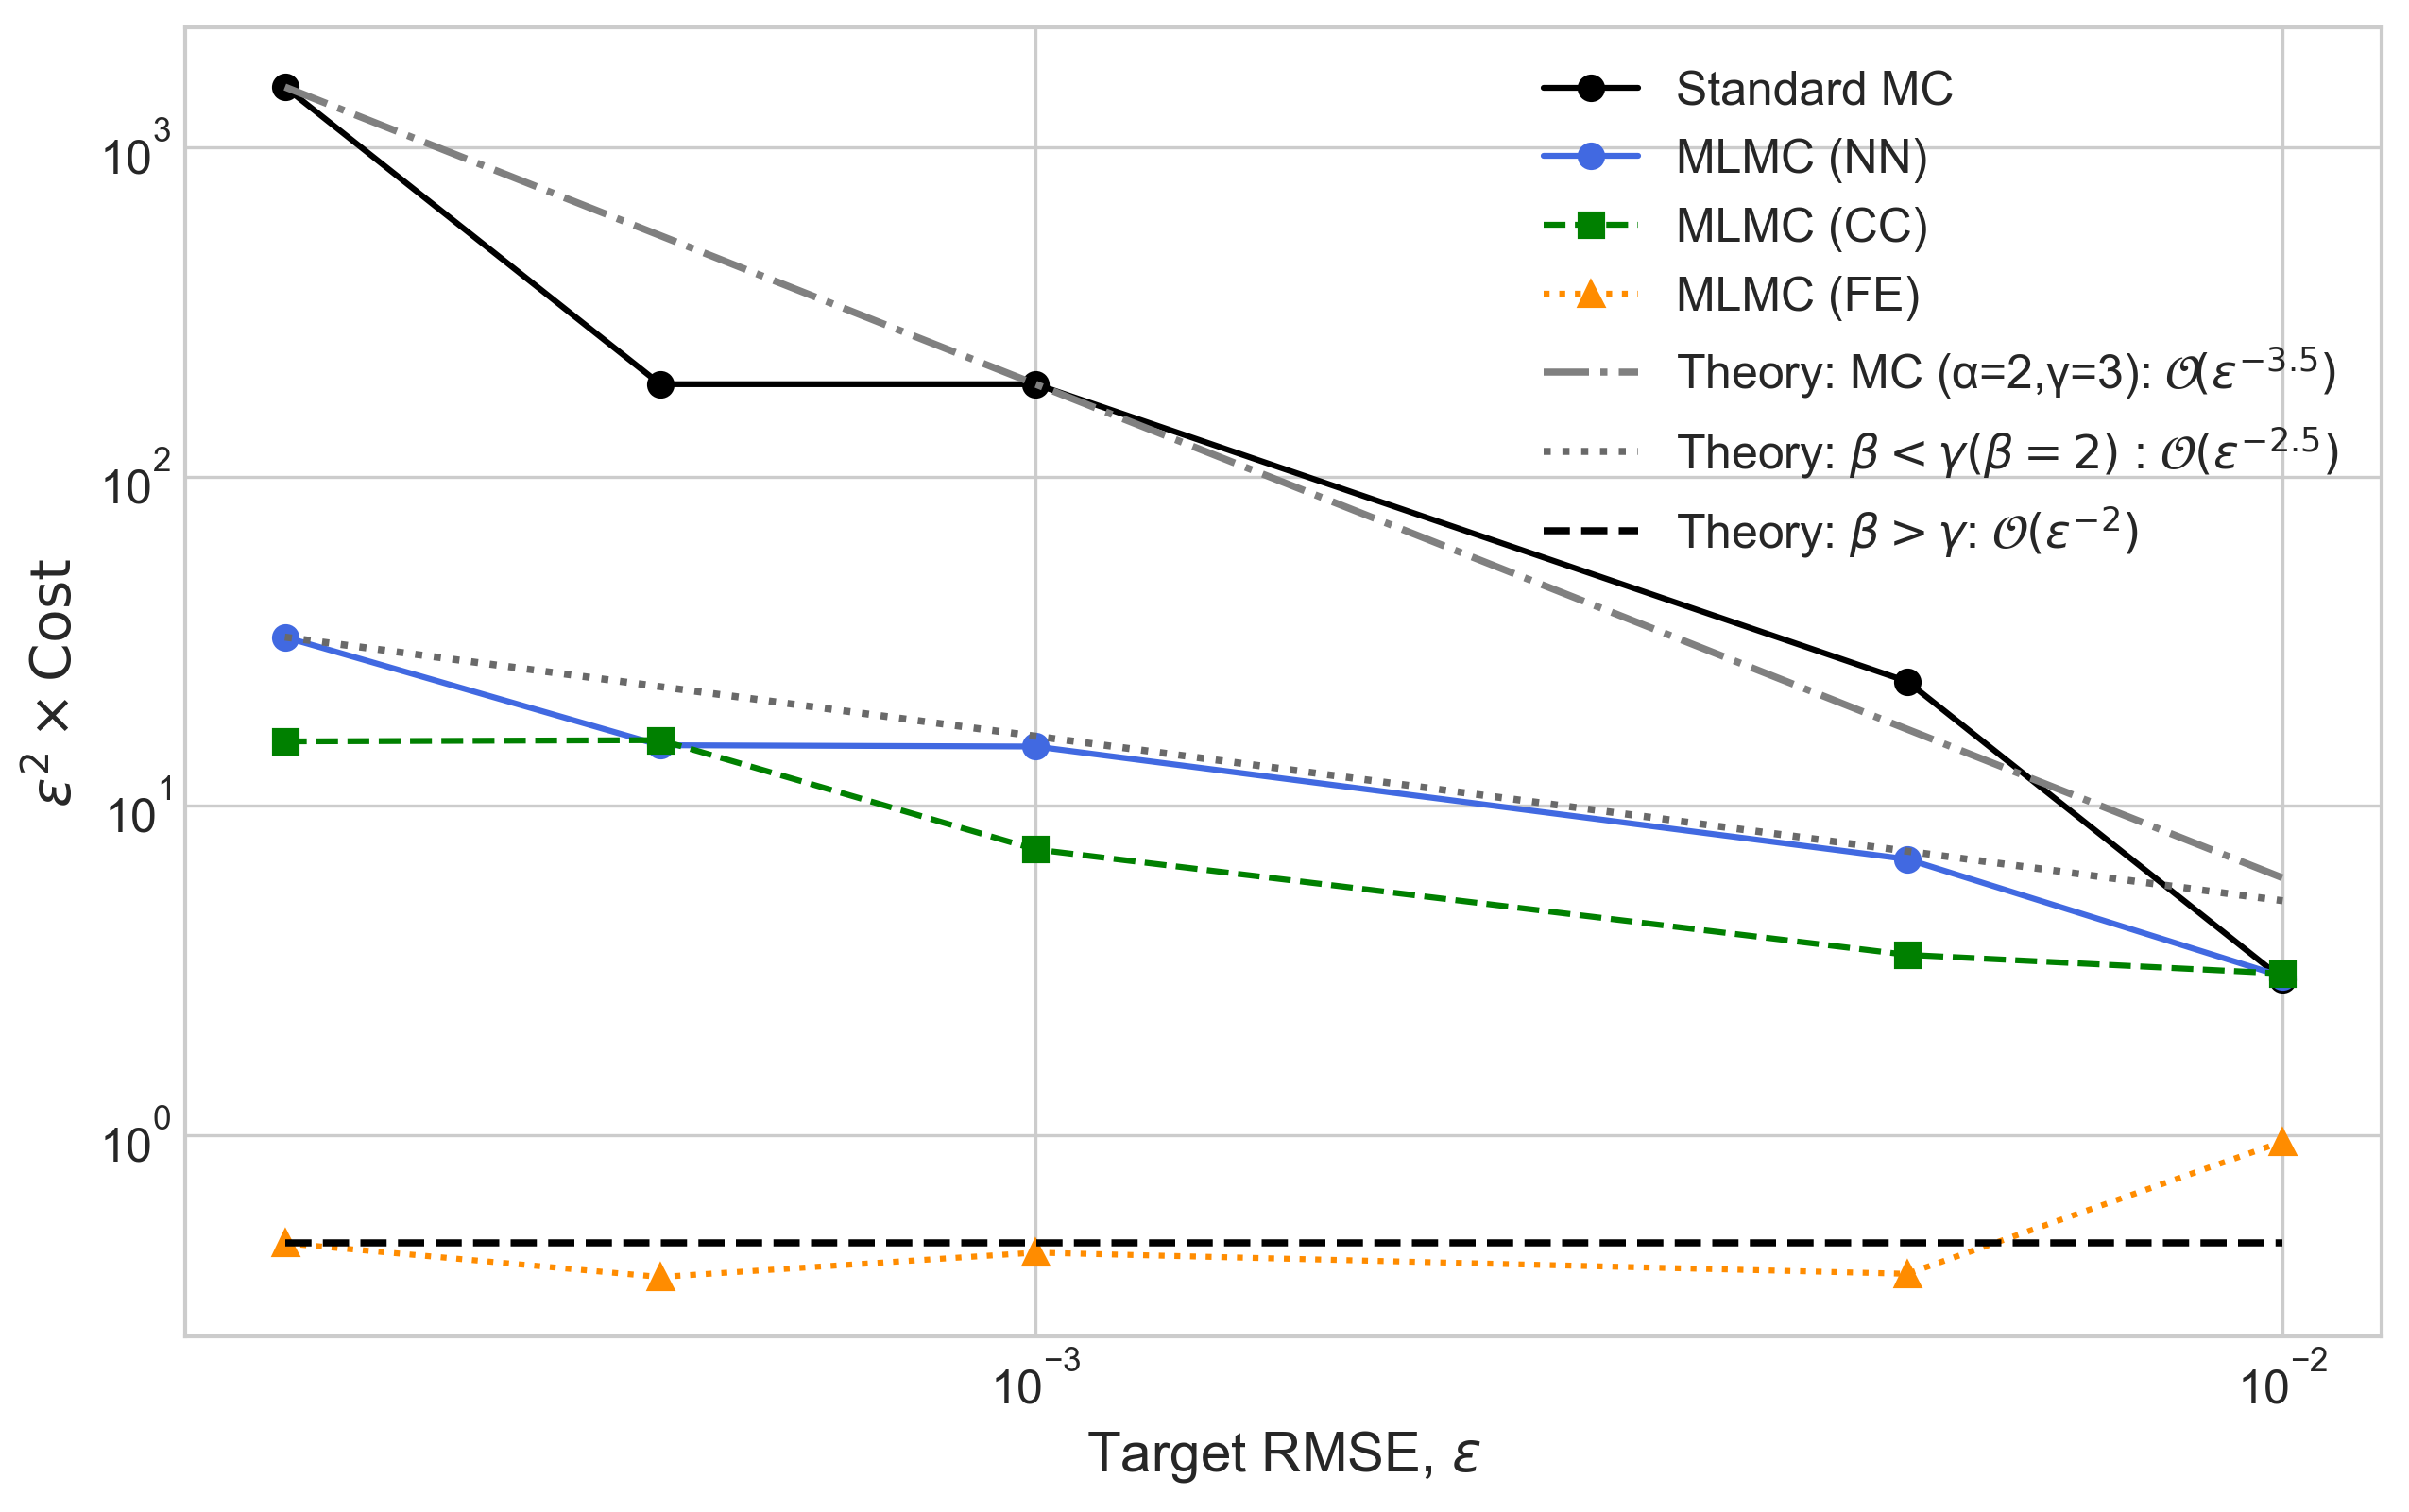
\includegraphics[height=2.7cm]{presentation_graphics/she_sq_amp_costs.png}
            {\scriptsize SHE - Squared Amplitude}
            \begin{itemize}\tiny
                \item FE coupling: optimal scaling $\mathcal{O}\left(\varepsilon^{-2}\right)$.
                \item NN and CC: both suboptimal  - $\mathcal{O}(\varepsilon^{-2-(\gamma-\beta) / \alpha})$.
            \end{itemize}
        \end{column}

        \begin{column}{0.32\textwidth}
            \centering
            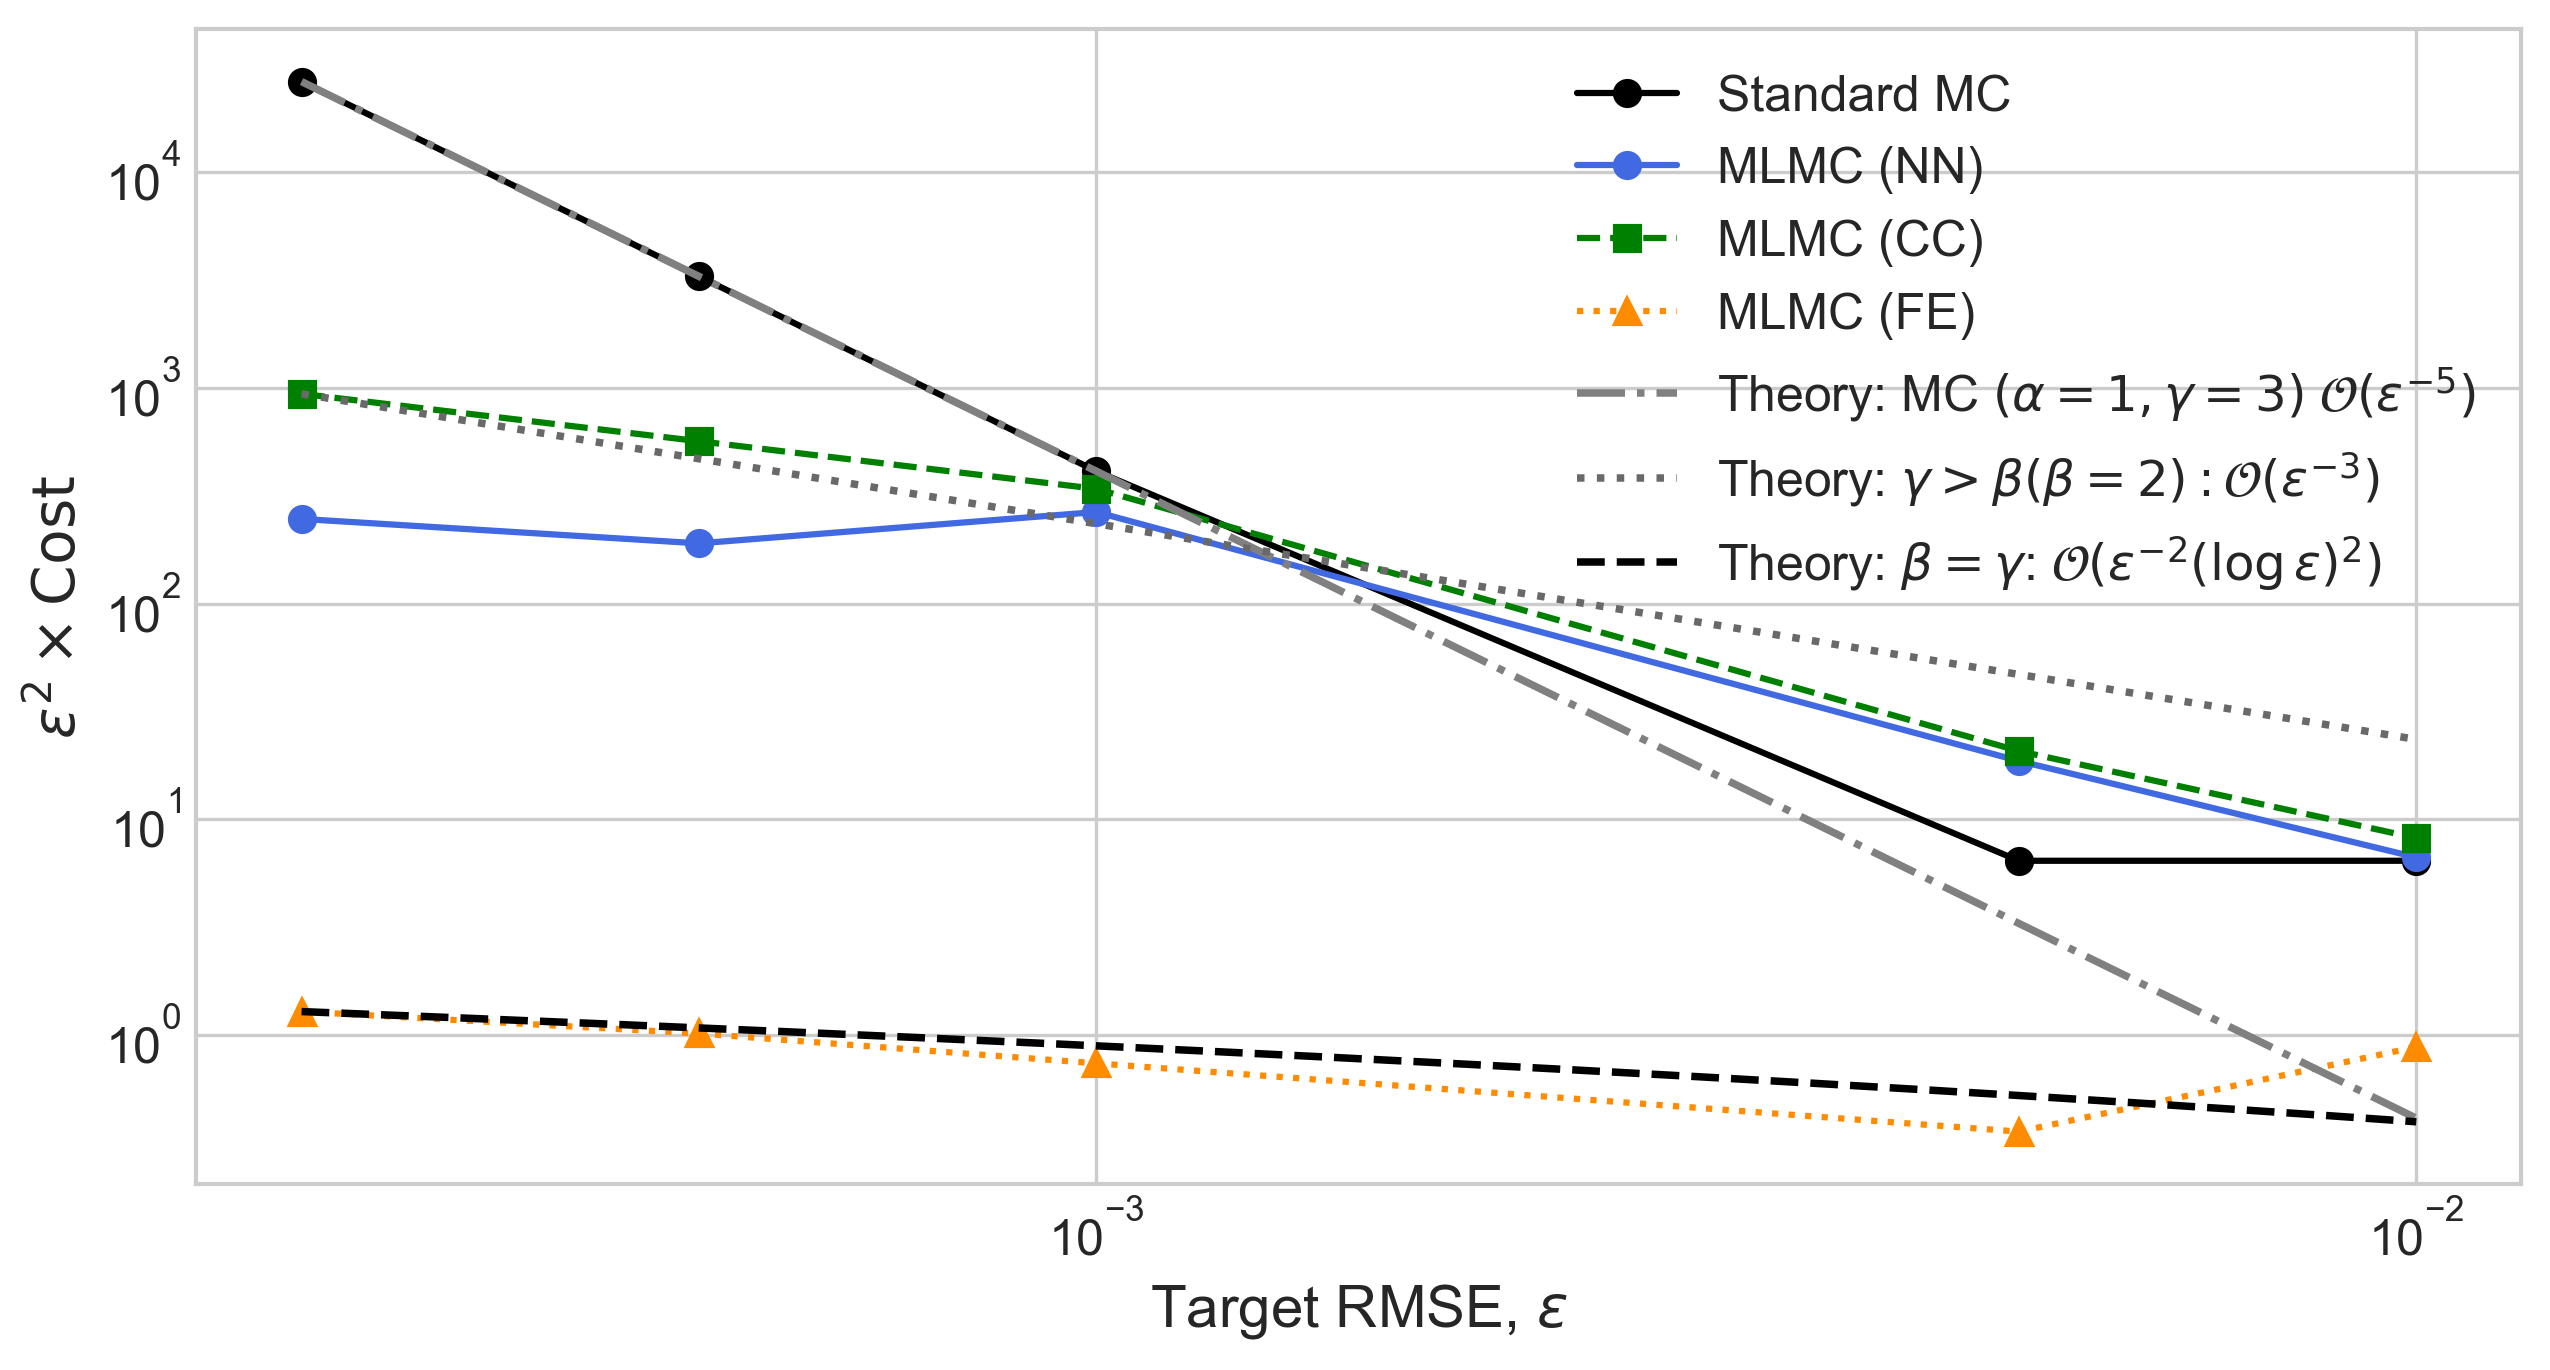
\includegraphics[height=2.7cm]{presentation_graphics/she_costs_energy.png}
            {\scriptsize SHE - Energy}
            \begin{itemize}\tiny
                \item FE coupling: near-optimal $\mathcal{O}\left(\varepsilon^{-2}(\log \varepsilon)^2\right)$.
                \item NN and CC: both suboptimal $\mathcal{O}(\varepsilon^{-2-(\gamma-\beta) / \alpha})$.
            \end{itemize}
        \end{column}

        \begin{column}{0.32\textwidth}
            \centering
            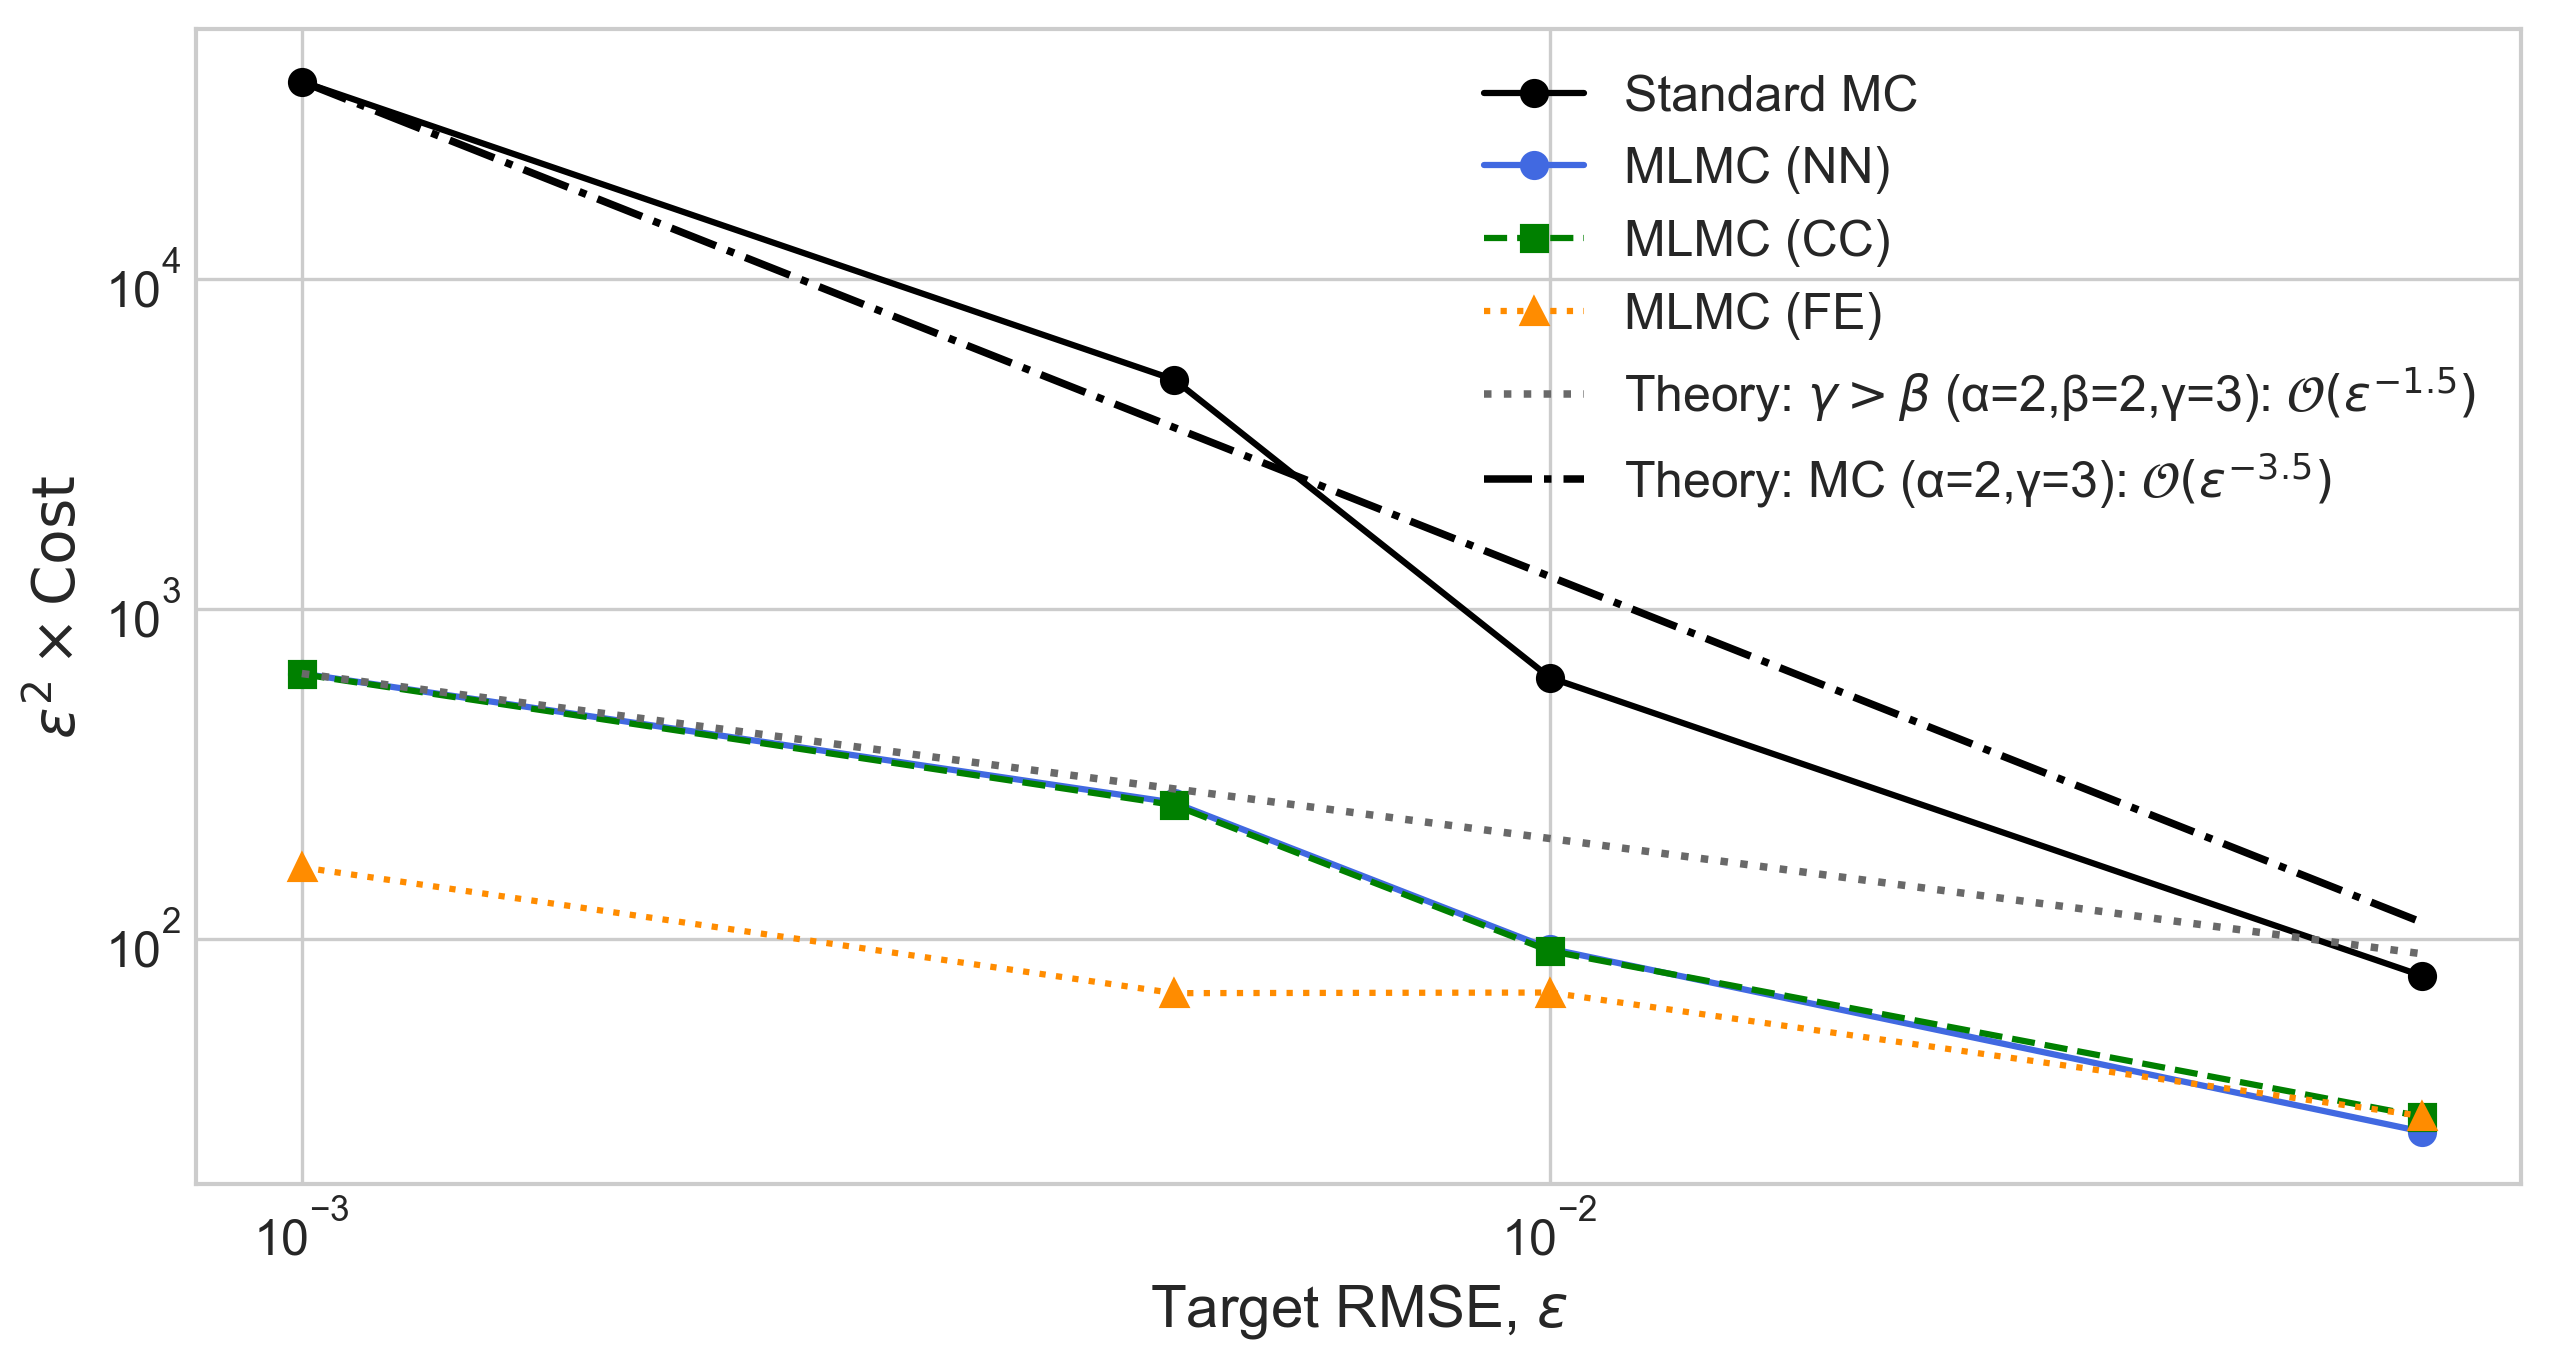
\includegraphics[height=2.7cm]{presentation_graphics/dk_costs.png}
            {\scriptsize DK - Mean Fluctuations}
            \begin{itemize}\tiny
                \item FE, NN and CC: equivalent scaling $\mathcal{O}(\varepsilon^{-2-(\gamma - \beta) / \alpha})$.
            \end{itemize}
        \end{column}
    \end{columns}
\end{frame}

\begin{frame}{Parallelism in MLMC}
\centering
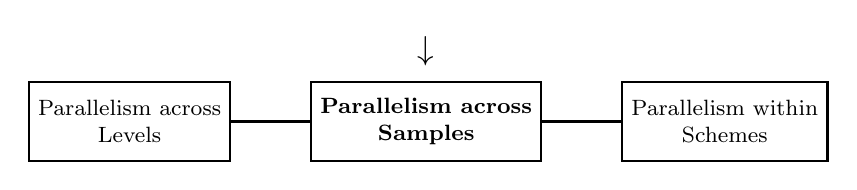
\begin{tikzpicture}[
  node distance = 1cm, 
  block/.style = {
    draw, rectangle, thick,
    minimum width=2cm, minimum height=1.0cm, 
    align=center,
    font=\footnotesize
  }
]

\node[block] (levels) {Parallelism across \\ Levels};
\node[block, right = of levels] (samples) {\textbf{Parallelism across} \\ \textbf{Samples}};
\node[block, right = of samples] (schemes) {Parallelism within \\ Schemes};

\draw[-, thick] (levels.east) -- (samples.west);
\draw[-, thick] (samples.east) -- (schemes.west);

\node[black, above=0.06cm of samples] {\scalebox{1.2}{$\downarrow$}};

\end{tikzpicture}

\begin{columns}[T] % The [T] option top-aligns the columns

    \begin{column}{0.6\textwidth}
        \vspace{3.6em}
        \begin{itemize}
            \item Parallelised MLMC algorithm over samples using OpenMP.
            \item Resulted in baseline average $\times 4$ speed improvement.
        \end{itemize}
    \end{column}

    % --- Right Column for the Graphic ---
    \begin{column}{0.4\textwidth}
        % The \centering command is optional but good practice
        \centering
        % \linewidth makes the image fit the column width
        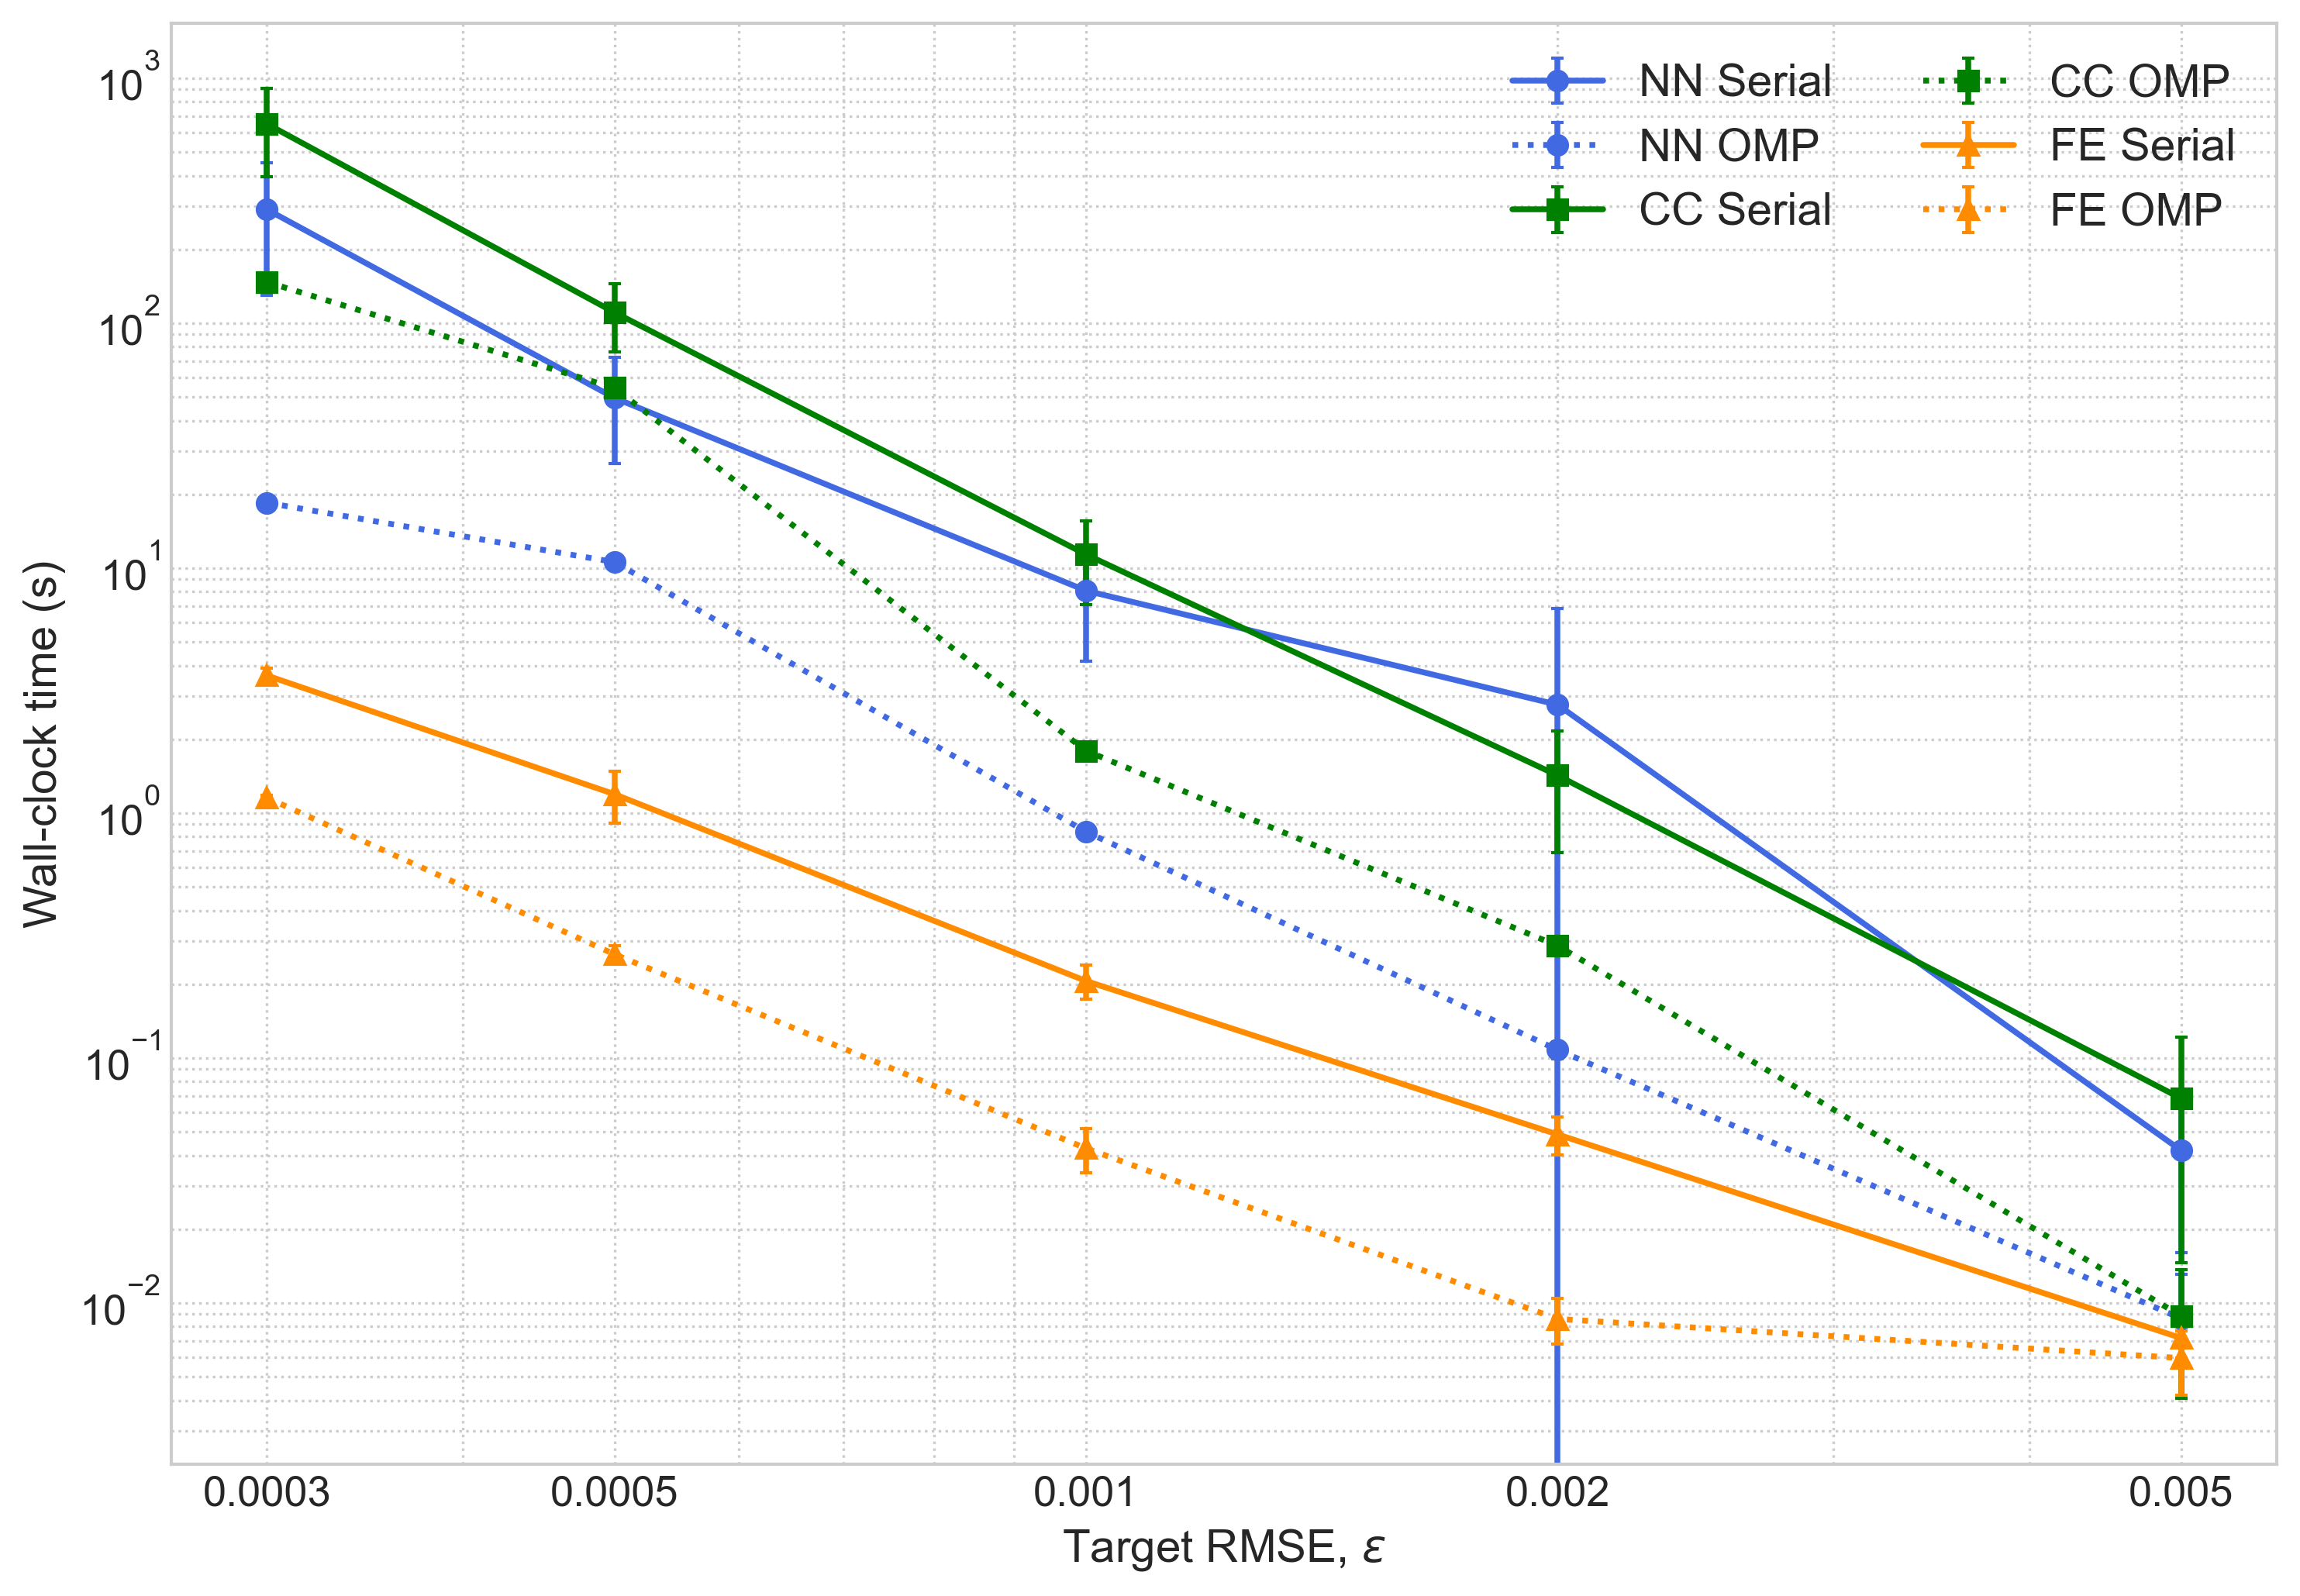
\includegraphics[width=\linewidth]{presentation_graphics/perf_wallclock_vs_eps.png}
    \end{column}

\end{columns}
\end{frame}

\begin{frame}{}
\centering
\quad Thank you for listening.
\newline

\qquad Questions?

\end{frame}



% \begin{frame}{FE Coupling for DK equations}
    \scriptsize
    Let $\phi$ be the hat basis functions, and our approximate
    solution be 
    $\rho(t, x) = \sum_{j=1}^{J-1} \rho_j(t) \phi_j(x)$.

    \begin{align*}
        \left(\frac{\partial \rho}{\partial t}, \phi_i\right)_{\Delta x} 
        &= 
        \frac{1}{2}\left(\frac{\partial^2 \rho}{\partial t^2}, 
        \phi_i\right)_{\Delta x}
        + N_p^{-1/2}
        \left(\frac{\partial \sqrt{\rho} \xi}{\partial x}, \phi_i\right)_{\Delta x}
        &&
        \text{(Inner product)}
        \\
        M \mathrm{d}\boldsymbol{\rho}(t) + 
        &\frac{1}{2}K \boldsymbol{\rho}(t)\mathrm{d}t 
        = 
        \mathrm{d}\boldsymbol{\eta}
        \\
        \int_0^{2 \pi} \frac{\partial (\sqrt{\rho}\xi)}{\partial x} \phi_i \mathrm{d}x
        &=-\int_{x_i - \Delta x}^{x_i + \Delta x}\sqrt{\rho}\xi \phi_i' \mathrm{d}x
        = -\int_{x_i - \Delta x}^{x_i} \sqrt{\rho}\xi \frac{1}{\Delta x} dx
        + \int_{x_i}^{x_i+\Delta x} \sqrt{\rho}\xi \frac{1}{\Delta x} dx,
        \quad \phi_i' = 
        \begin{cases}
            \frac{1}{\Delta x}, \quad x \in [x_i - \Delta x, x_i]\\
            \frac{-1}{\Delta x}, \quad x \in [x_i, x_i + \Delta x]\\
        \end{cases}
        \\
        &= \frac{F_{i+1/2} - F_{i-1/2}}{\Delta x}, \quad F_{i+1/2} := 
    \end{align*}
\end{frame}


\end{document}
